\chapter{Keep it Organized}
\label{chap:KeepitOrganized}


In each project do any or preferably all of 
the following. They may be inconvenient during
the daily routine work. They, however, can save you 
a lot of time in rare events. Some events
frequently occur where the price is low. Some events
occurs rarely with a high price.
An irrelevant example is ``extreme weather events are 
low-probability high impact events'' in power grid systems.
In our case, there might come a time that you need
to look back and figure out what you did and why you did
it a few months ago. Keeping a \emph{diary} can save you 
a lot of headache.
\begin{enumerate}
\item The easiest way of keeping your project flow organized is to 
include a numeric part in the name of files and folders.
For example, \codeGreen{01\_FetchData\_from\_GEE.py} can be the name
of your first script with the same or similar name for the folder 
(\code{user/document/projectXYX/\hl{01\_Data\_from\_GEE}/}) for the data coming from this step; \code{Data\_from\_GEE.csv}. 

Then, \codeGreen{02\_remove\_noise.py},
\codeGreen{03\_regression\_smooth\_data.py}, \codeGreen{04\_plot\_the\_result.py},
\codeGreen{04\_analyze\_the\_result.py}.

Note that I have two items starting with ``04\_''. 
These two are independent of each other
and both depend on ``\codeGreen{03\_regression\_smooth\_data.py}''.

\item Include dates in your codes. On top of the code
document the dates and that helps you to see what you did last
if you need to dig in the history and re-do stuff.

\item If you want to be on top of things, you can create 
something like~\cref{Workflow,WorkflowZoom}. An end-to-end 
flowchart/doodle of the workflow.

\begin{figure}[htb]
  \centering
  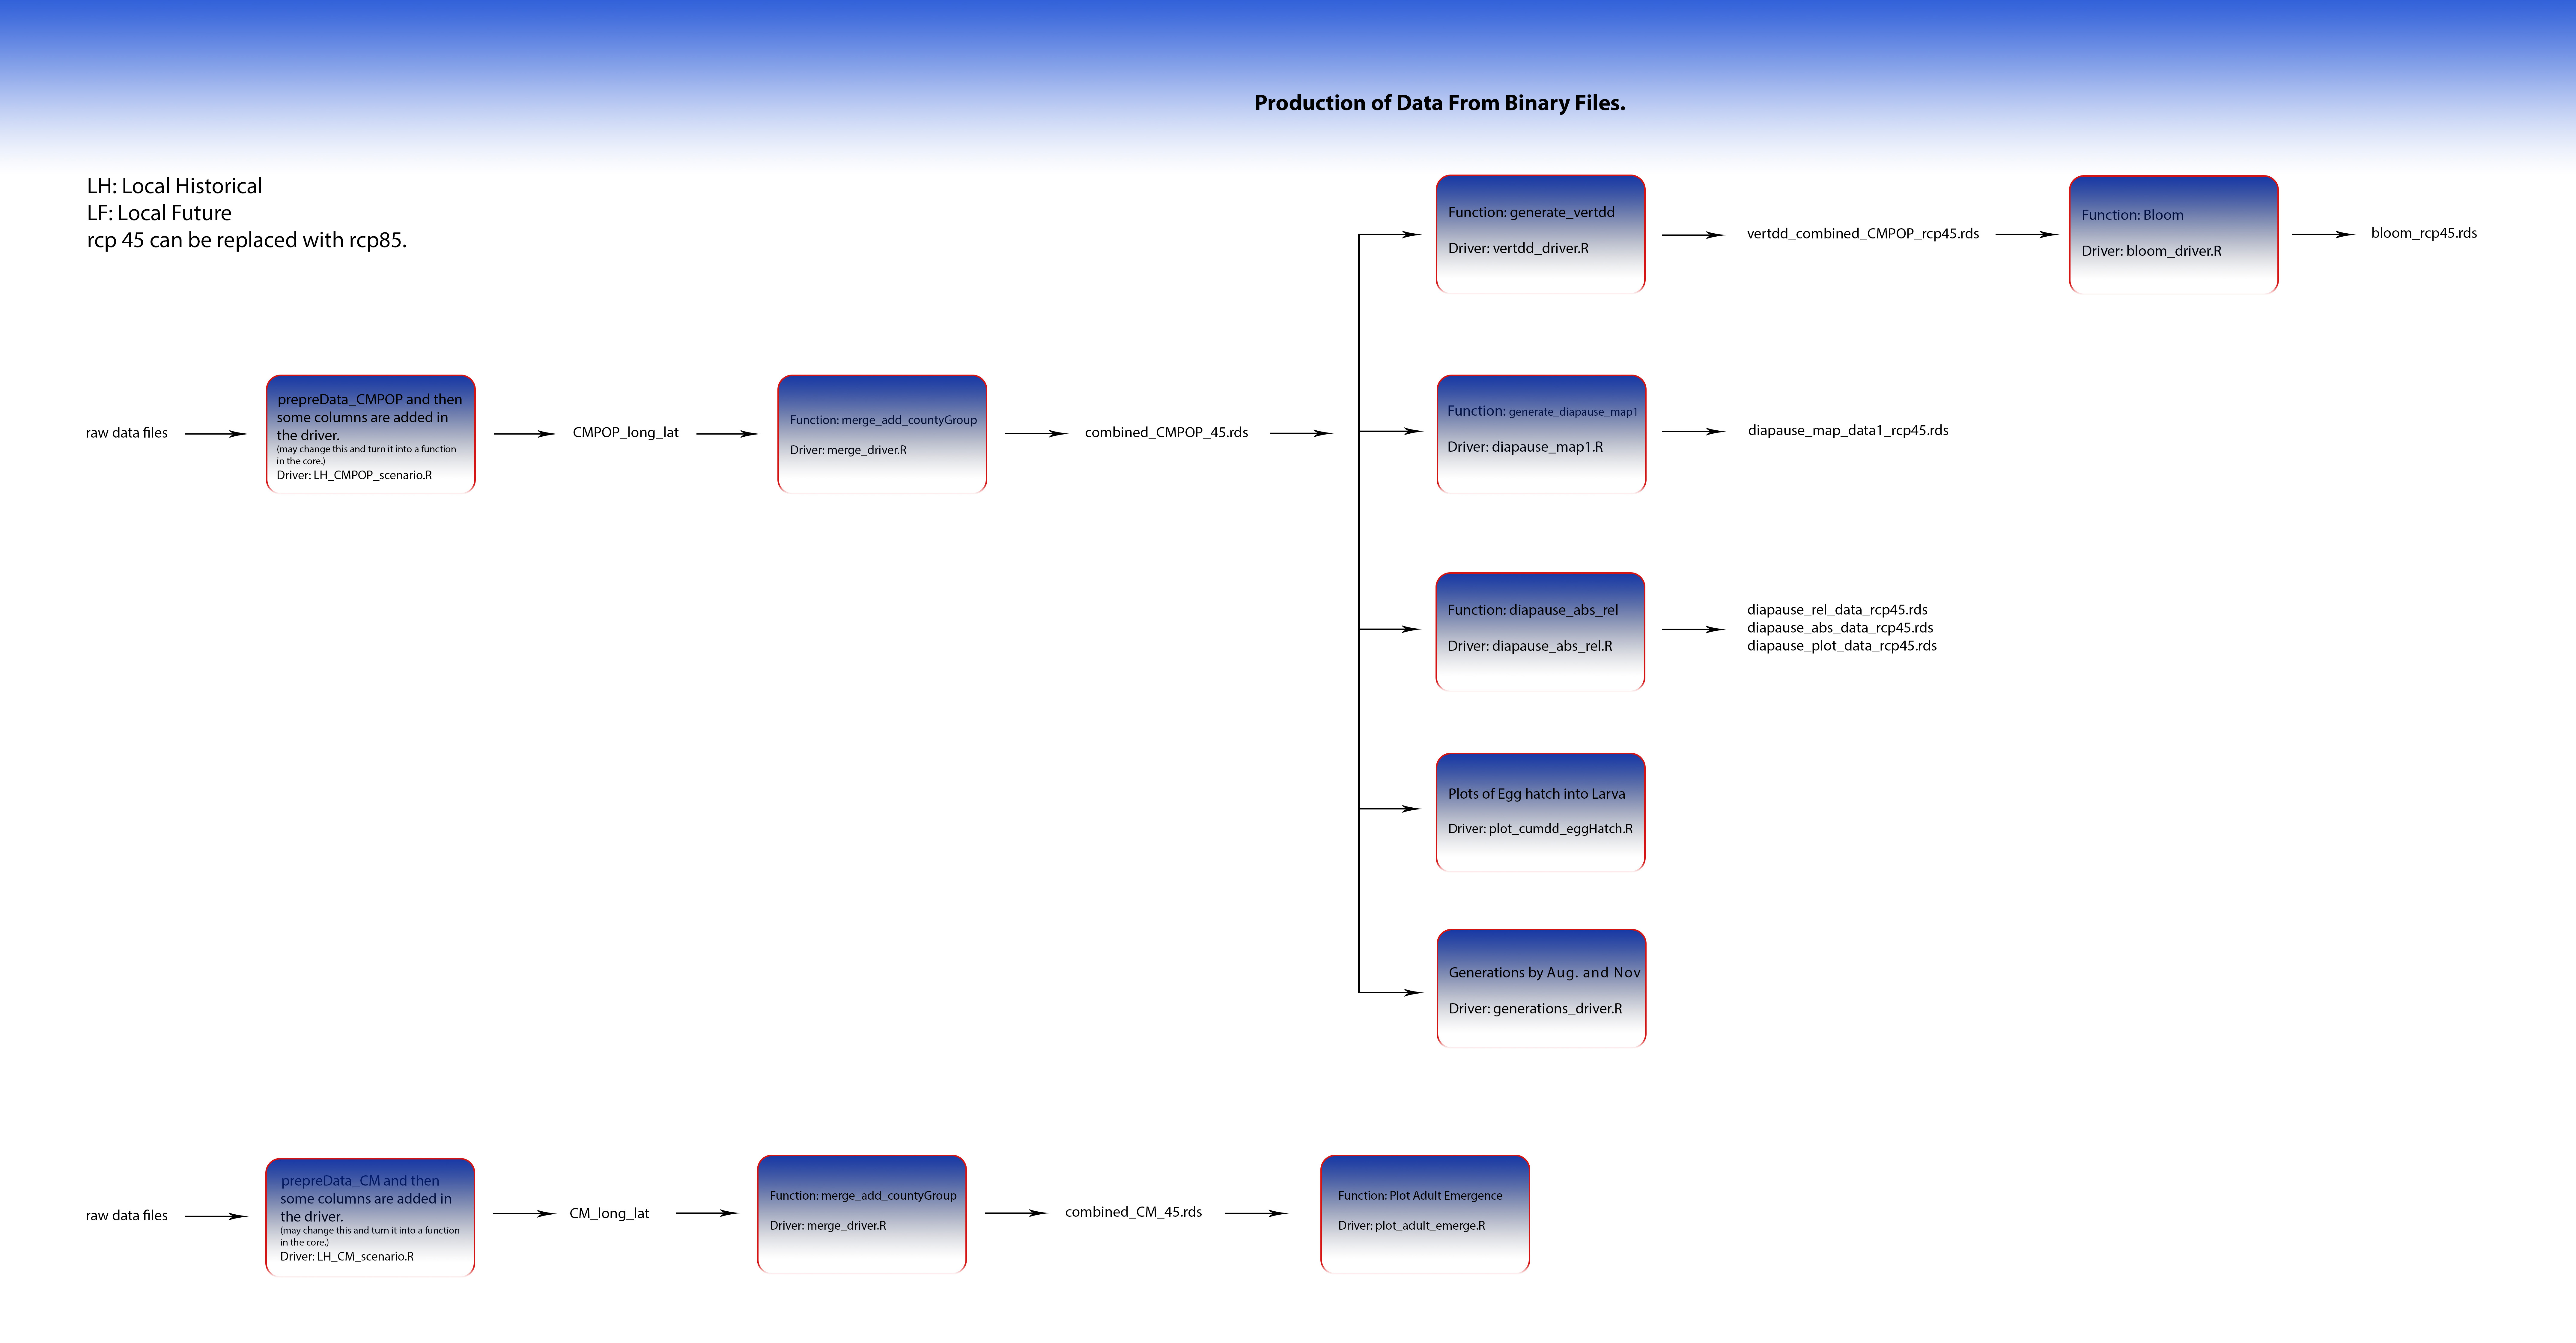
\includegraphics[width=1\textwidth]{figures/pipe_Line}
  \caption{Workflow for one of my projects.}
  \label{Workflow}
\end{figure}

\begin{figure}[htb]
  \centering
  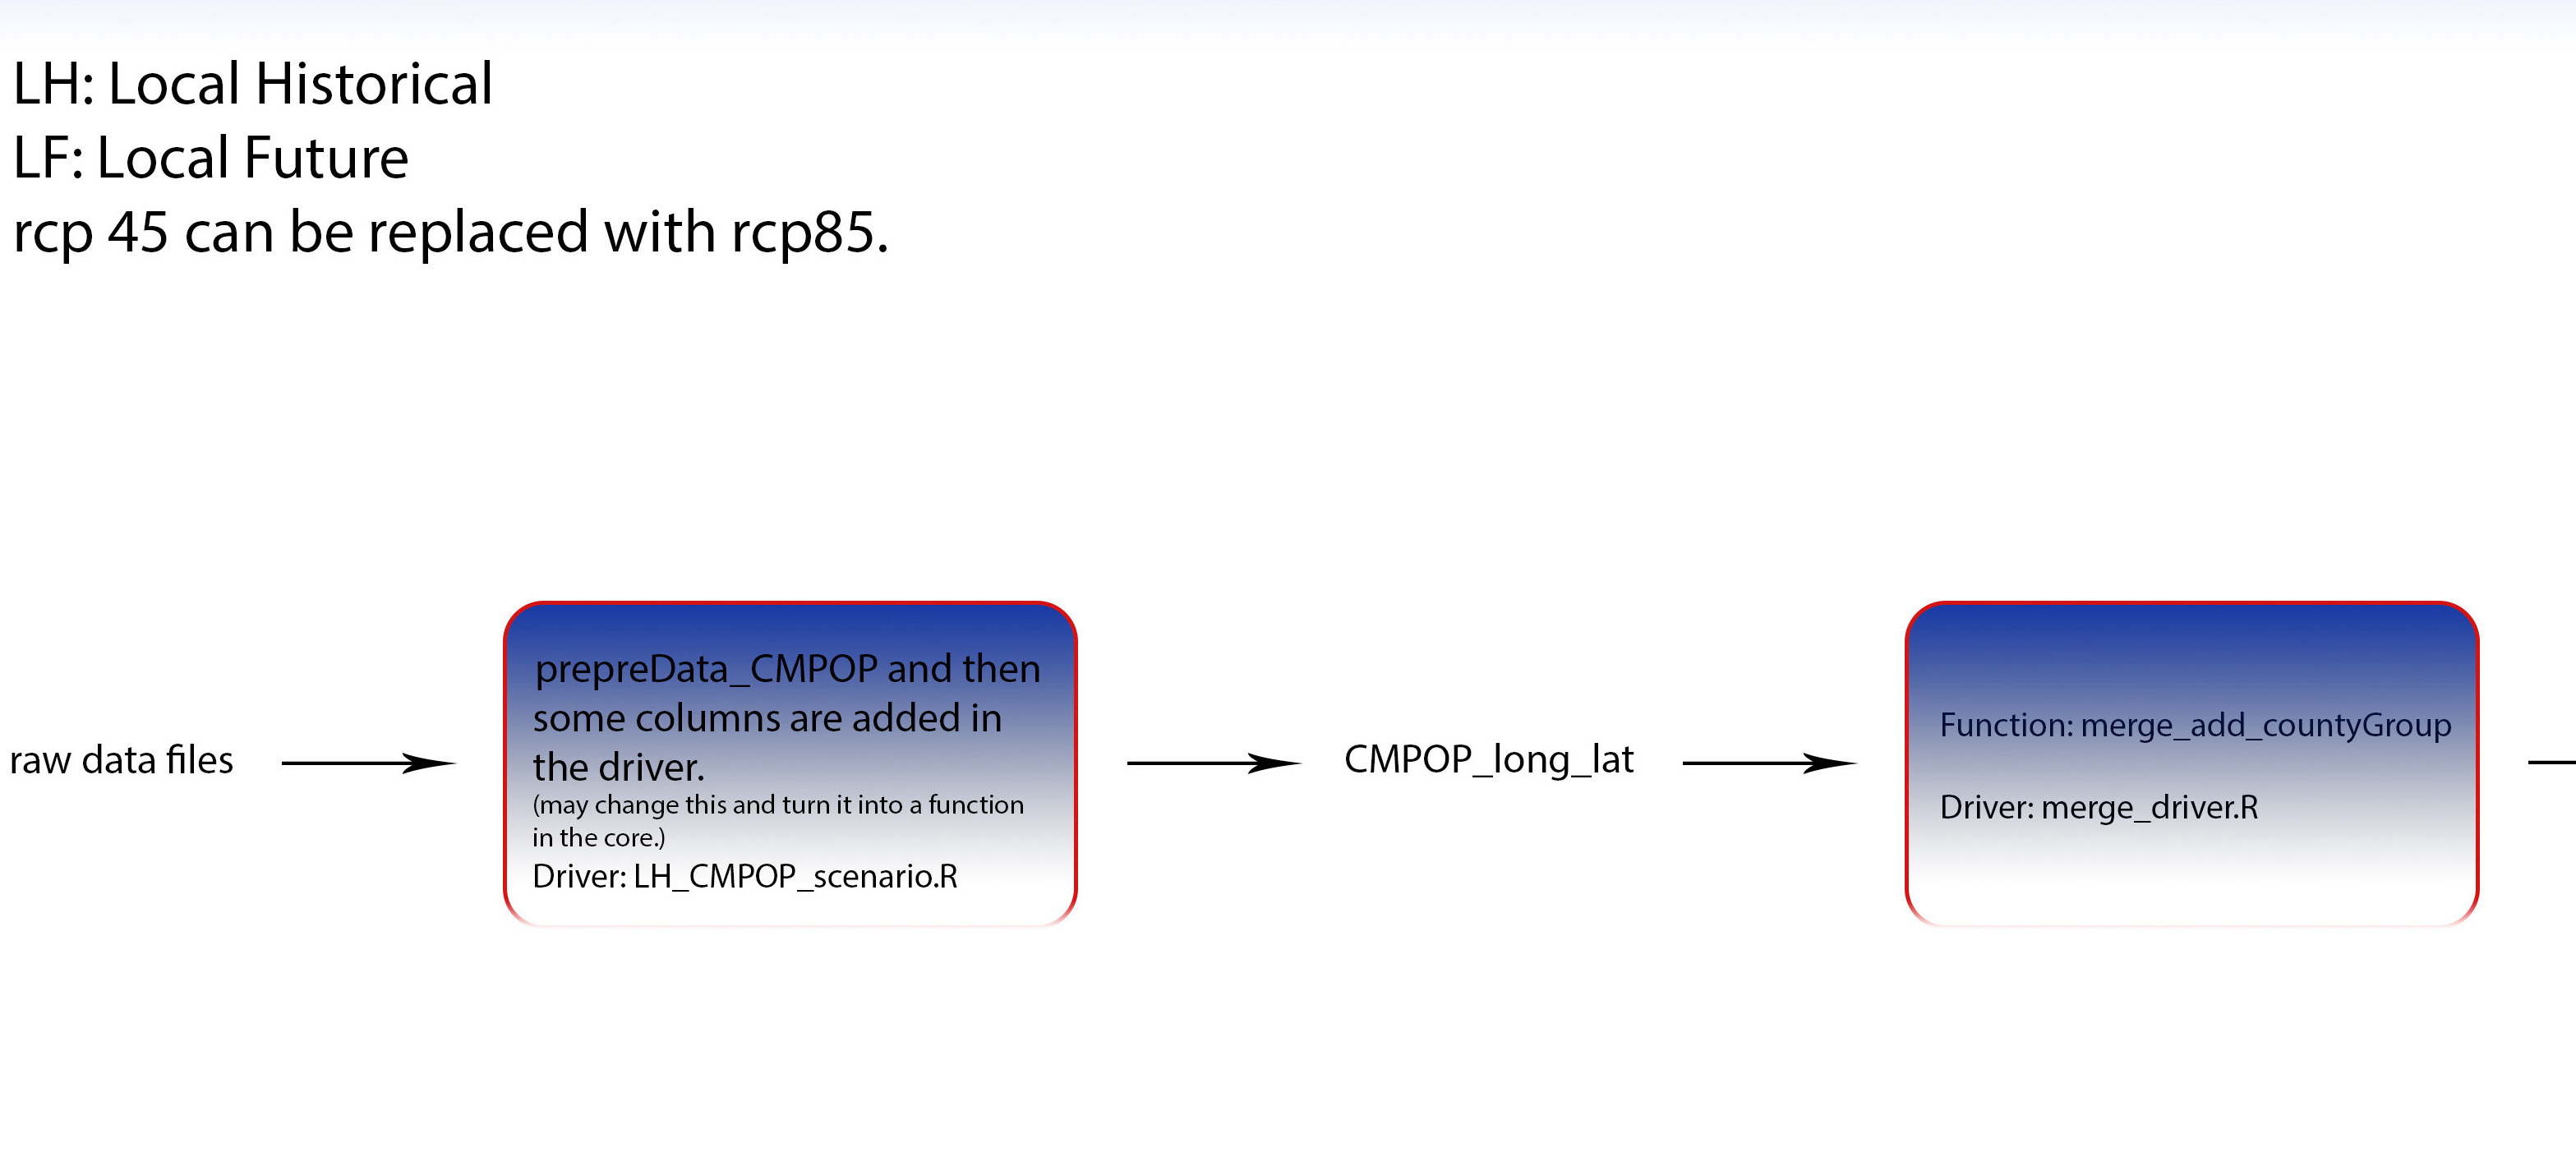
\includegraphics[width=1\textwidth]{figures/pipe_Line_zoom}
  \caption{Workflow zoomed in.}
  \label{WorkflowZoom}
\end{figure}





\end{enumerate}